\documentclass[border=4pt,varwidth=17cm]{standalone}
\usepackage{amsmath,amssymb,mathrsfs,mathtools}
\usepackage{tikz}
\usetikzlibrary{positioning,fit,backgrounds,arrows.meta}
\def\RR{{\mathbb R}}\def\eps{\varepsilon}\def\then{\Rightarrow}
\def\J{\mathcal{J}_L}\def\A{\mathcal{A}_{f,g}}\def\Sol{\mathcal{S}_{f,g}}
\def\limsup{\mathop{\overline{\lim}}}\def\liminf{\mathop{\underline{\lim}}}
\def\Of{{\sf (O$_f$)}}\def\Og{{\sf (O$_g$)}}
\def\Rv{{\sf (R$_{\rm v}$)}}\def\Rh{{\sf (R$_{\rm h}$)}}
\begin{document}


\scalebox{0.93}{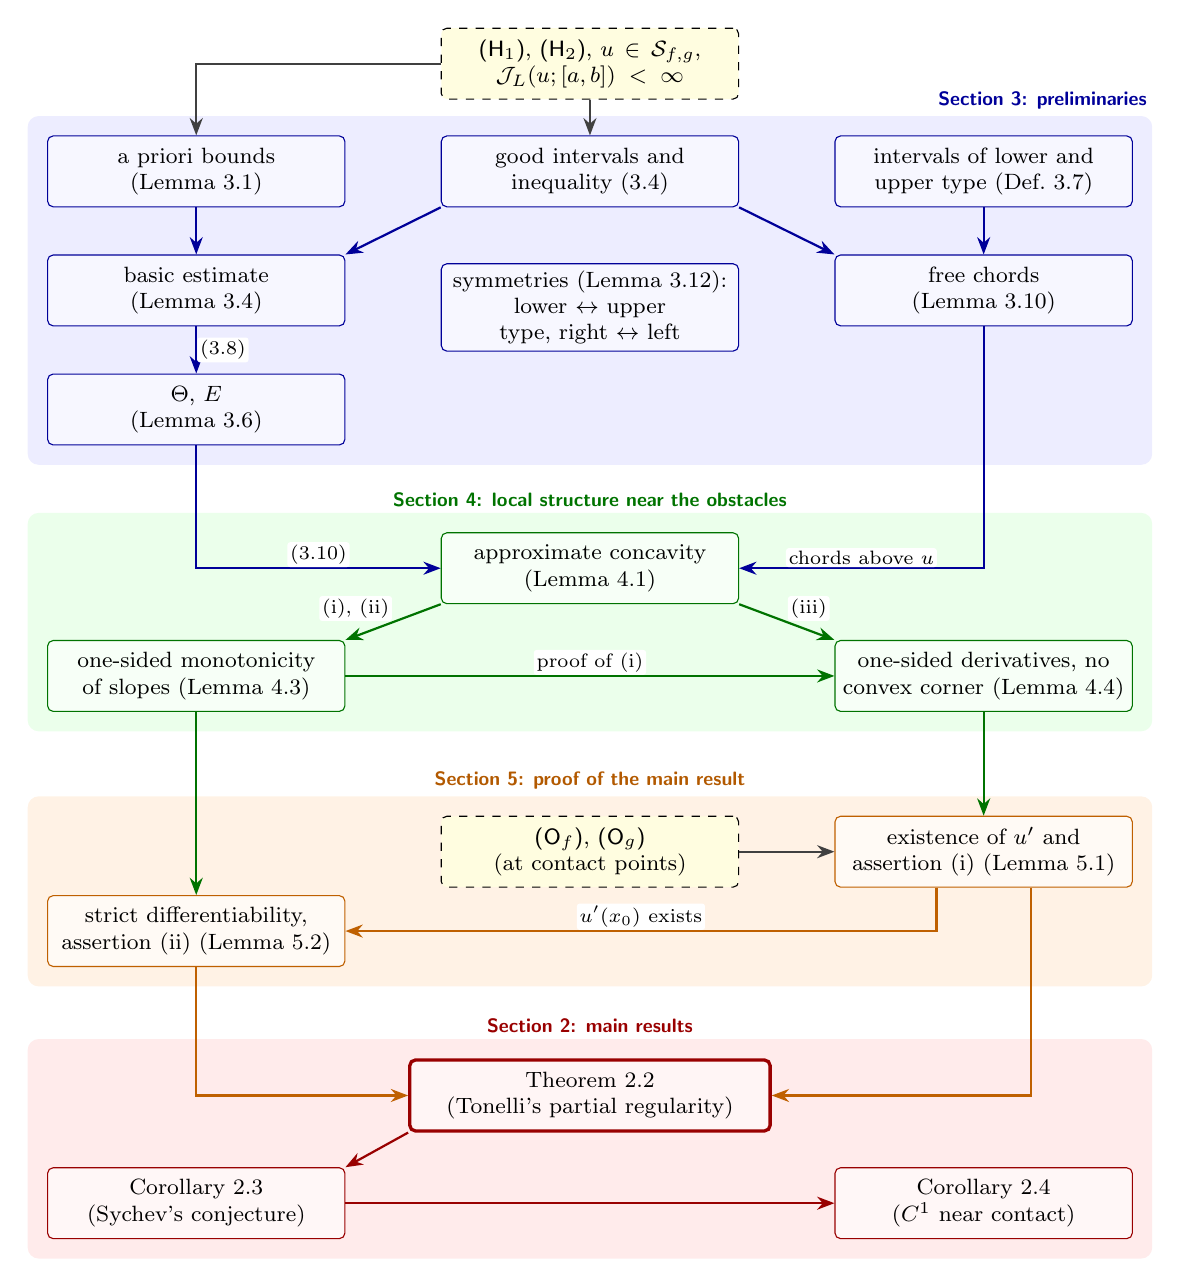
\begin{tikzpicture}[y=0.72cm,
  font=\footnotesize,
  box/.style={draw, rounded corners=2pt, fill=white, align=center, text width=3.6cm, minimum height=0.9cm, inner sep=2.5pt},
  hyp/.style={box, dashed, fill=yellow!12},
  main/.style={box, very thick, draw=red!60!black, fill=red!4},
  arr/.style={-{Stealth[length=2.2mm]}, thick, draw=black!75},
  s3/.style={draw=blue!60!black, fill=blue!3},
  s4/.style={draw=green!45!black, fill=green!3},
  s5/.style={draw=orange!75!black, fill=orange!4},
  s2/.style={draw=red!60!black, fill=red!3},
  a3/.style={arr, draw=blue!60!black},
  a4/.style={arr, draw=green!45!black},
  a5/.style={arr, draw=orange!75!black},
  a2/.style={arr, draw=red!60!black},
  lab/.style={font=\scriptsize, fill=white, rounded corners=1pt, inner sep=1pt},
  band/.style={fill=gray!10, rounded corners=4pt, inner sep=7pt},
  bandtitle/.style={font=\scriptsize\bfseries\sffamily, anchor=south east, inner sep=2pt}
]
% hypotheses
\node[hyp] (H) at (5,1.9) {{\sf (H$_1$)}, {\sf (H$_2$)}, $u\in\Sol$,\\ $\J(u;[a,b])<\infty$};
% Section 3
\node[box, s3] (A) at (0,0) {a priori bounds\\(Lemma~3.1)};
\node[box, s3] (B) at (5,0) {good intervals and inequality (3.4)};
\node[box, s3] (C) at (10,0) {intervals of lower and upper type (Def.~3.7)};
\node[box, s3] (D) at (0,-2.1) {basic estimate\\(Lemma~3.4)};
\node[box, s3] (S) at (5,-2.4) {symmetries (Lemma~3.12): lower $\leftrightarrow$ upper type, right $\leftrightarrow$ left};
\node[box, s3] (F) at (10,-2.1) {free chords\\(Lemma~3.10)};
\node[box, s3] (T) at (0,-4.2) {$\Theta$, $E$\\(Lemma~3.6)};
% Section 4
\node[box, s4] (G) at (5,-7.0) {approximate concavity\\(Lemma~4.1)};
\node[box, s4] (M1) at (0,-8.9) {one-sided monotonicity of slopes (Lemma~4.3)};
\node[box, s4] (I) at (10,-8.9) {one-sided derivatives, no convex corner (Lemma~4.4)};
% Section 5
\node[hyp] (O) at (5,-12.0) {\Of, \Og\\(at contact points)};
\node[box, s5] (J) at (10,-12.0) {existence of $u^\prime$ and assertion (i) (Lemma~5.1)};
\node[box, s5] (K) at (0,-13.4) {strict differentiability, assertion (ii) (Lemma~5.2)};
% Section 2
\node[main, text width=4.4cm] (Th) at (5,-16.3) {Theorem~2.2\\(Tonelli's partial regularity)};
\node[box, s2] (C1) at (0,-18.2) {Corollary~2.3\\(Sychev's conjecture)};
\node[box, s2] (C2) at (10,-18.2) {Corollary~2.4\\($C^1$ near contact)};
% bands
\begin{scope}[on background layer]
  \node[band, fill=blue!7, fit=(A)(B)(C)(D)(S)(F)(T)] (b3) {};
  \node[band, fill=green!8, fit=(G)(M1)(I)] (b4) {};
  \node[band, fill=orange!10, fit=(O)(J)(K)] (b5) {};
  \node[band, fill=red!8, fit=(Th)(C1)(C2)] (b2) {};
\end{scope}
\node[bandtitle, text=blue!60!black] at (b3.north east) {Section~3: preliminaries};
\node[bandtitle, anchor=south, text=green!45!black] at (b4.north) {Section~4: local structure near the obstacles};
\node[bandtitle, anchor=south, text=orange!70!black] at (b5.north) {Section~5: proof of the main result};
\node[bandtitle, anchor=south, text=red!60!black] at (b2.north) {Section~2: main results};
% arrows
\draw[arr] (H) -| (A);
\draw[arr] (H) -- (B);
\draw[a3] (A) -- (D);
\draw[a3] (B.south west) -- (D.north east);
\draw[a3] (B.south east) -- (F.north west);
\draw[a3] (C) -- (F);
\draw[a3] (D) -- node[lab, right] {(3.8)} (T);
\draw[a3] (T) |- node[lab, pos=0.75, above] {(3.10)} (G);
\draw[a3] (F) |- node[lab, pos=0.75, above] {chords above $u$} (G);
\draw[a4] (G.south west) -- node[lab, above left] {(i), (ii)} (M1.north east);
\draw[a4] (G.south east) -- node[lab, above right] {(iii)} (I.north west);
\draw[a4] (M1) -- node[lab, above] {proof of (i)} (I);
\draw[a4] (I) -- (J);
\draw[arr] (O) -- (J);
\draw[a4] (M1) -- (K);
\draw[a5] ([xshift=-6mm]J.south) |- node[lab, pos=0.75, above] {$u^\prime(x_0)$ exists} (K.east);
\draw[a5] ([xshift=6mm]J.south) |- (Th.east);
\draw[a5] (K) |- (Th.west);
\draw[a2] (Th.south west) -- (C1.north east);
\draw[a2] (C1) -- (C2);
\end{tikzpicture}}


\end{document}
